\chapter*{Proposition 23}
\label{prop:23}

\begin{figure*}[ht]
    \begin{center}
    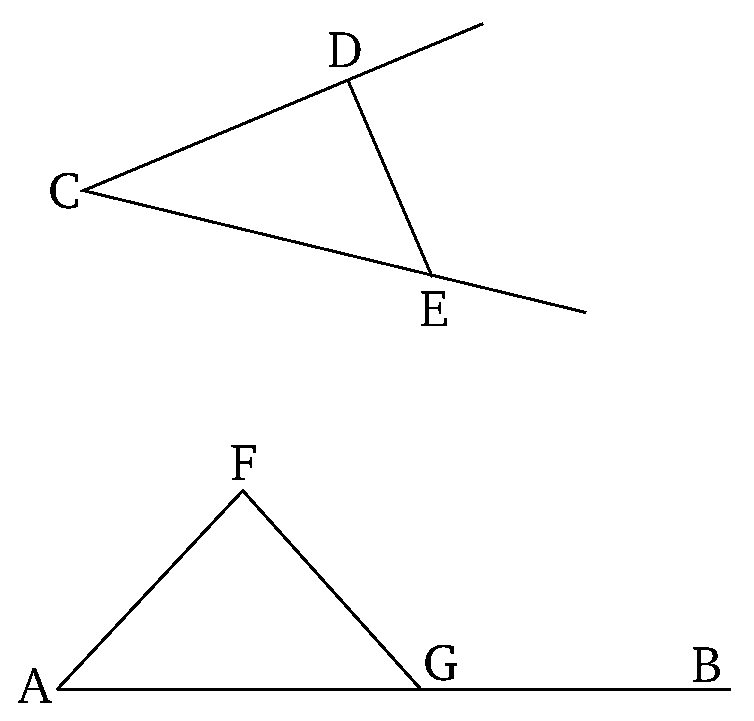
\includegraphics[width=0.5\linewidth]{figures/fig23e.eps}
    \label{fig:prop_23}
    \end{center}
\end{figure*}

To construct a rectilinear angle equal to a given rectilinear angle at a (given)
point on a given straight-line.\\

Let $AB$ be the given straight-line,  $A$ the (given) point on it, and 
$DCE$ the given rectilinear angle. So it is required to construct a rectilinear
angle equal to the given rectilinear angle $DCE$ at the (given) point
$A$ on the given straight-line
$AB$.

Let the points $D$ and $E$ have been taken at random on each
of the (straight-lines) $CD$ and $CE$ (respectively), and let $DE$ have been joined.
And let the triangle $AFG$ have been constructed from three straight-lines
which are equal to $CD$, $DE$, and $CE$, such that $CD$ is equal to $AF$,
$CE$ to $AG$, and further $DE$ to $FG$ [Prop.~1.22].

Therefore, since the two (straight-lines) $DC$, $CE$ are equal to the
two (straight-lines) $FA$, $AG$, respectively, and the base $DE$ is equal to
the base $FG$, the angle $DCE$ is thus equal to the angle $FAG$ [Prop.~1.8].

Thus, the rectilinear angle $FAG$,  equal to the  given
rectilinear angle $DCE$, has been constructed at the (given) point $A$ on the given straight-line $AB$.
(Which is) the very thing it was required to do.


\section*{Commentary}

\begin{proposition}\label{proposition_23}\lean{Elements.Book1.proposition_23}\leanok
    $\angle~DCE$ is an angle. $A$ and $B$ are two distinct points on a line $AB$. Then, there must exists a point $F$ different from $A$, s.t., $\angle~FAB = \angle~DCE$.
\end{proposition}
\begin{proof}
    \uses{proposition_8,proposition_20,proposition_22'}\leanok
    Euclid's proof omitted the degenerated cases that $D$ is on $CE$, i.e., $\angle~DCE$ is either $0$ or $\pi$.
    In addition, when constructing $\triangle~AFG$, Euclid didn't prove that such a triangle can be constructed from $CD$, $CE$, and $DE$, which can be done by applying Proposition~\ref{proposition_20}.
\end{proof}

Euclid didn't prove that $F$ can be constructed on either side of $AB$, which is useful for later proofs.

\begin{proposition}\label{proposition_23'}\lean{Elements.Book1.proposition_23'}\leanok
    $\angle~DCE$ is an angle. $A$ and $B$ are two distinct points on a line $AB$. $X$ is a point not on $AB$. Then, there must exists a point $F$ different from $A$, s.t., $\angle~FAB = \angle~DCE$, and $F$ is either on $AB$ or on the same side of $AB$ with $X$.
\end{proposition}
\begin{proof}
    \uses{proposition_8,proposition_20,proposition_22''}\leanok
    Similar to the previous proof.
\end{proof}